\documentclass{article}

% NeurIPS 2024 style — preprint mode (non-anonymous, for arXiv)
\usepackage[preprint]{neurips_2024}

\usepackage[utf8]{inputenc}
\usepackage[T1]{fontenc}
\usepackage{hyperref}
\usepackage{url}
\usepackage{booktabs}
\usepackage{amsfonts}
\usepackage{amsmath}
\usepackage{amssymb}
\usepackage{nicefrac}
\usepackage{microtype}
\usepackage{graphicx}
\usepackage{xcolor}
\usepackage{array}
\usepackage{tabularx}

\graphicspath{{figures/}}

\title{Scale Collapse, Model Disagreement, and False Precision:\\
A Multi-Model Audit of LLM Behavioral Interview Scoring}

\author{%
  Kewen Zhu \\
  \And
  Ze Sheng \\
  \And
  Zixi Liu \\
  \And
  Junyuan Tan \\
}

\begin{document}

\maketitle

\begin{abstract}
Large Language Models (LLMs) are increasingly deployed as hiring evaluators, yet no systematic reliability audit exists for this high-stakes domain. We benchmark 9 frontier models from 3 families (GPT-5.4, Claude, Gemini) across 10 behavioral questions, 3 companies, and 2 seniority levels (141 cells, 10--50 samples each, 4{,}600 total ratings), revealing five reliability failures: (1) \textbf{Scale collapse}~--- a 5-point scale degenerates into 2.03 effective categories (normalized entropy $=0.44$); (2) \textbf{Test--retest unreliability}~--- ICC(2,1) ranges from 0.16 to 0.85 across models; (3) \textbf{Inter-model disagreement}~--- Krippendorff's $\alpha = 0.52$, below the 0.67 tentative-conclusion threshold, with same-brand variants (Spearman $\rho=0.25$) disagreeing more than cross-vendor pairs ($\rho=0.87$); (4) \textbf{Question-type sensitivity}~--- identical answers receive ratings differing by 2 ordinal grades across question types; (5) \textbf{Expectation gap}~--- community-endorsed answers score below ``Hire'' across all models, with flagship models significantly harsher than lightweight (Wilcoxon $z=-2.80$, $p=.005$). We propose a minimum reliability checklist and discuss implications for AI hiring policy.
\end{abstract}

\textbf{Keywords:} LLM Evaluation Reliability; AI-Assisted Hiring; Behavioral Interviews; Multi-Model Benchmark; Algorithmic Auditing; Scale Collapse.

\section{Introduction}

\subsection{Background: The Rise of AI in Hiring}
Artificial intelligence is rapidly transforming hiring practices. An estimated 99\% of Fortune~500 companies now use AI-powered tools somewhere in their recruitment pipeline, and 90\% of large employers use automated systems to filter job applications~\cite{allaboutai2025}. SHRM's 2024 Talent Trends Survey found that among organizations using AI for HR, 64\% apply it to recruitment, interviewing, and hiring --- the leading use case~\cite{shrm2024}. Products like HireVue, Pymetrics, and numerous startup offerings promise to evaluate candidates at scale using Large Language Models (LLMs). The appeal is clear: consistent evaluation, reduced human bias, faster throughput, and lower cost per assessment.

The behavioral interview --- in which candidates describe past experiences demonstrating competencies such as leadership, conflict resolution, and problem-solving --- is a cornerstone of hiring at major technology companies including Google, Meta, and Amazon. These companies employ structured rubrics to evaluate behavioral answers on ordinal scales, making them a natural target for LLM-based automation.

\subsection{The Missing Audit}
Despite rapid deployment, a critical gap exists: \textbf{no systematic reliability audit has been conducted on LLM behavioral interview evaluators}. This stands in stark contrast to other high-stakes AI applications:
\begin{itemize}
  \item Medical AI systems require FDA clearance and clinical validation before deployment.
  \item Financial AI models undergo rigorous backtesting and stress testing.
  \item Criminal justice risk assessment tools face increasing scrutiny and auditing requirements.
\end{itemize}
Yet AI hiring tools --- which directly affect people's livelihoods --- operate with minimal reliability benchmarking. The few existing studies focus on single-model evaluations or narrow prompt engineering without addressing fundamental questions of measurement reliability.

\subsection{Research Questions}
We address three core questions:
\begin{enumerate}
  \item \textbf{Scale utilization:} Do LLM evaluators effectively use the full range of hiring rating scales, or does the scale degenerate under automated evaluation?
  \item \textbf{Reliability:} How consistent are LLM hiring ratings across repeated evaluations (test--retest) and across different models (inter-rater)?
  \item \textbf{Validity:} Do LLM ratings align with community expectations for behavioral interview answer quality?
\end{enumerate}

\subsection{Contributions}
\begin{enumerate}
  \item \textbf{The first multi-model behavioral interview scoring benchmark}, spanning 9 frontier models, 3 model families, 3 companies, 2 seniority levels, and 10 behavioral questions, with up to 50 repeated samples per evaluation cell.
  \item \textbf{Five empirically validated reliability failures} in LLM interview scoring: scale collapse, test--retest unreliability, inter-model disagreement, question-type sensitivity, and expectation gap.
  \item \textbf{A model robustness scorecard} demonstrating that stability (self-consistency) and consensus (inter-model agreement) are orthogonal dimensions --- no single model excels on all reliability axes.
  \item \textbf{A minimum reliability checklist} for deploying LLM interview evaluators, informed by our empirical findings.
  \item \textbf{Open-source evaluation framework} enabling reproducible auditing of LLM interview scoring systems.
\end{enumerate}

\subsection{Paper Organization}
Section~\ref{sec:related} reviews related work. Section~\ref{sec:design} describes our experimental design. Section~\ref{sec:results} presents our five core findings. Section~\ref{sec:scorecard} introduces the model robustness scorecard. Section~\ref{sec:discussion} proposes the reliability checklist and discusses implications. Section~\ref{sec:limitations} acknowledges limitations. Section~\ref{sec:conclusion} concludes.

\section{Related Work}\label{sec:related}

\subsection{LLM-as-Judge}
The paradigm of using LLMs as evaluators has gained significant traction.~\cite{zheng2023} introduced MT-Bench and Chatbot Arena for evaluating conversational AI using LLM judges.~\cite{liu2023geval} proposed G-Eval, demonstrating that GPT-4 evaluations correlate with human judgments for text generation quality. However, these works focus on general NLG evaluation rather than domain-specific, high-stakes assessment.

Recent studies have identified systematic biases in LLM judges, including leniency bias~\cite{wang2024}, position bias~\cite{zheng2023}, and verbosity bias~\cite{saito2023}. Our work extends this line of inquiry to the hiring domain, where such biases have direct consequences for candidates and employers.

\subsection{AI in Hiring}
Automated hiring systems have evolved from keyword-matching resume screeners to sophisticated multi-modal assessment platforms. HireVue (now part of the broader AI hiring ecosystem) processes millions of video interviews annually. Academic work has explored automated interview scoring~\cite{naim2018,hemamou2019} and feedback generation~\cite{hoque2013}.

However, the reliability of these systems remains underexplored.~\cite{raghavan2020} surveyed AI hiring tools and found a lack of validation evidence.~\cite{wilson2021} highlighted fairness concerns in AI hiring but did not conduct systematic reliability auditing. Our work fills this gap with the first multi-model reliability benchmark specifically for behavioral interview evaluation.

\subsection{Evaluation Reliability in Psychology}
The psychometric tradition provides a rigorous framework for evaluating measurement instruments. Key reliability dimensions include:
\begin{itemize}
  \item \textbf{Test--retest reliability:} Consistency of scores across repeated measurements~\cite{cronbach1951}.
  \item \textbf{Inter-rater reliability:} Agreement among different raters evaluating the same subject~\cite{shrout1979}.
  \item \textbf{Internal consistency:} Coherence of items within a scale~\cite{mcdonald1999}.
\end{itemize}
We adapt these classical reliability frameworks to the LLM evaluation context, treating each model as a ``rater'' and each repeated API call as a ``retest.''

\subsection{Regulatory Landscape}
The regulatory environment for AI hiring is rapidly evolving:
\begin{itemize}
  \item \textbf{NYC Local Law 144} requires annual bias audits for automated employment decision tools~\cite{nyc2023}.
  \item \textbf{Illinois AI Video Interview Act} mandates disclosure when AI analyzes video interviews~\cite{illinois2020}.
  \item \textbf{EU AI Act} classifies AI hiring tools as ``high-risk,'' requiring conformity assessments~\cite{euaiact2024}.
  \item \textbf{EEOC} guidance addresses AI-related discrimination in employment decisions~\cite{eeoc2023}.
  \item \textbf{NIST AI Risk Management Framework} provides standards for high-risk AI applications~\cite{nist2023}.
\end{itemize}
Our work provides empirical evidence directly relevant to these regulatory requirements, demonstrating specific failure modes that auditing frameworks should address.

\subsection{Positioning}
Our work differs from prior studies in several key respects: (1) we evaluate multiple frontier models from different vendors rather than a single model; (2) we focus specifically on behavioral interview evaluation, a high-stakes domain with structured rubrics; (3) we apply psychometric reliability frameworks (test--retest, inter-rater agreement) rather than focusing solely on accuracy; (4) we conduct the evaluation at scale (141 cells, up to 50 samples each) to enable robust statistical analysis.

\section{Experimental Design}\label{sec:design}

\subsection{Answer Source: Community Consensus Baseline}
We use 10 behavioral interview question--answer pairs from the \textit{awesome-behavioral-interviews} GitHub repository, a curated resource with over 8{,}000 stars --- one of the most popular behavioral interview preparation resources on the internet. We selected this source deliberately: these answers represent \textbf{community consensus on what constitutes a ``good'' behavioral interview answer}. With 8{,}000+ stars, they reflect a broad ``sounds reasonable'' crowd endorsement, making them an ideal baseline for testing whether LLM evaluators agree with community expectations.

\begin{table}[h]
\caption{Question categories covered in the benchmark.}
\label{tab:categories}
\centering
\begin{tabular}{lll}
\toprule
\textbf{Category} & \textbf{Questions} & \textbf{N} \\
\midrule
Vulnerability & Failure, conflict, pressure, tough feedback, manager disagreement & 5 \\
Leadership & Led a team, difficult decision & 2 \\
Initiative & Above and beyond & 1 \\
Epistemic & Handle not knowing the answer & 1 \\
Introduction & Tell me about yourself & 1 \\
\bottomrule
\end{tabular}
\end{table}

\subsection{Model Matrix}
We evaluate 9 models from 3 major LLM provider families, covering the full capability-cost spectrum (Table~\ref{tab:models}). Flagship models receive 10 samples per cell due to higher cost; lightweight and mid-tier models receive 50 samples for richer distribution estimates. All models were accessed via LiteLLM with temperature $=0$ (or minimum available) for evaluation consistency.

\begin{table}[h]
\caption{Model matrix: 9 frontier models across 3 families.}
\label{tab:models}
\centering
\begin{tabular}{llll}
\toprule
\textbf{Family} & \textbf{Model} & \textbf{Tier} & \textbf{Samples/Cell} \\
\midrule
OpenAI GPT-5.4 & gpt-5.4 & Mid & 10 \\
 & gpt-5.4-pro & Flagship & 10 \\
 & gpt-5.4-mini & Lightweight & 50 \\
Anthropic Claude & claude-opus-4-6 & Flagship & 10 \\
 & claude-sonnet-4-6 & Mid & 50 \\
 & claude-haiku-4-5 & Lightweight & 50 \\
Google Gemini & gemini-3.1-pro-preview & Flagship & 10 \\
 & gemini-3-flash-preview & Mid & 50 \\
 & gemini-3.1-flash-lite-preview & Lightweight & 50 \\
\bottomrule
\end{tabular}
\end{table}

\subsection{Evaluation Dimensions}
Each answer is evaluated under 6 configurations (3 companies $\times$ 2 levels):
\begin{itemize}
  \item \textbf{Companies:} Google, Meta, Amazon --- representing distinct but overlapping behavioral interview cultures.
  \item \textbf{Levels:} Mid-level, Senior --- reflecting different expectation bars.
\end{itemize}
This yields 141 unique evaluation cells (question $\times$ company $\times$ level $\times$ model), as not all models were evaluated under all configurations due to cost optimization. The primary evaluation slice is \textbf{Google, Senior}, which has full 11-model coverage.

\subsection{Prompt Design}
We use a unified evaluation prompt across all models to ensure comparability:

\begin{quote}
\small\ttfamily
You are an interviewer at \{company\}.\\
Evaluate the candidate's behavioral answer for a \{level\} Software Engineer role.\\[2pt]
Question: \{question\}\\
Candidate answer: \{answer\}\\[2pt]
Output MUST be valid JSON:\\
\{"feedback": "<\textasciitilde 200 words>", "rating": "<No Hire $|$ Leaning No Hire $|$\\
\phantom{\{}Leaning Hire $|$ Hire $|$ Strong Hire>"\}
\end{quote}

The 5-point ordinal scale maps to: No Hire (1), Leaning No Hire (2), Leaning Hire (3), Hire (4), Strong Hire (5).

\subsection{Repeated Sampling and Test--Retest Protocol}
Each evaluation cell receives 10--50 independent API calls. For test--retest analysis, we conducted 27 separate experimental runs across different dates, allowing us to compute within-run and across-run agreement rates.

\subsection{Metrics}
We compute the following reliability metrics:
\begin{itemize}
  \item \textbf{Cell entropy} (Shannon entropy in nats): Measures rating distribution spread within a cell. Zero entropy = deterministic output.
  \item \textbf{Cross-question expected score SD:} Standard deviation of expected scores across questions for a given (company, level, model). Measures a model's sensitivity to question content.
  \item \textbf{Pairwise Spearman $\rho$:} Rank correlation of per-question expected scores between model pairs. Measures inter-model agreement on relative question difficulty.
  \item \textbf{Test--retest agreement rate:} Proportion of multi-replicate groups where all replicates yield the same rating.
  \item \textbf{Ordinal pstdev:} Population standard deviation of ordinal scores (1--5) within replicate groups.
\end{itemize}

In addition to these descriptive metrics, we apply formal statistical tests to quantify significance and effect size:
\begin{itemize}
  \item \textbf{Friedman test} ($\chi^2$): Non-parametric repeated-measures ANOVA testing whether models produce significantly different ratings across questions.
  \item \textbf{Kendall's W:} Coefficient of concordance measuring how consistently models rank-order questions from easiest to hardest.
  \item \textbf{ICC(2,1)}: Intraclass correlation coefficient (two-way random, single measures) quantifying test--retest reliability for each model.
  \item \textbf{Krippendorff's $\alpha$} (ordinal): Inter-model agreement metric suitable for ordinal data with any number of coders.
  \item \textbf{Wilcoxon signed-rank test:} Paired non-parametric test comparing flagship vs.\ lightweight model tiers on matched questions.
\end{itemize}

\section{Results: Five Reliability Failures}\label{sec:results}

\subsection{Finding 1: Scale Collapse --- A 5-Point Scale Used as a 2-Point Scale}

The most striking finding is the systematic collapse of the 5-point hiring scale. Across all 4{,}600 ratings (141 evaluation cells):
\begin{itemize}
  \item ``No Hire'' accounts for 0.0\% of ratings --- the lowest category is never assigned.
  \item ``Strong Hire'' accounts for only 0.43\% --- nearly absent.
  \item ``Leaning Hire'' dominates at 77.2\%, with ``Leaning No Hire'' at 14.0\% and ``Hire'' at 8.4\%.
  \item 62\% of cells have zero entropy --- the model produces the same rating every single time.
  \item 90--100\% of ratings concentrate in a single bin for the majority of cells.
\end{itemize}

\begin{figure}[h]
  \centering
  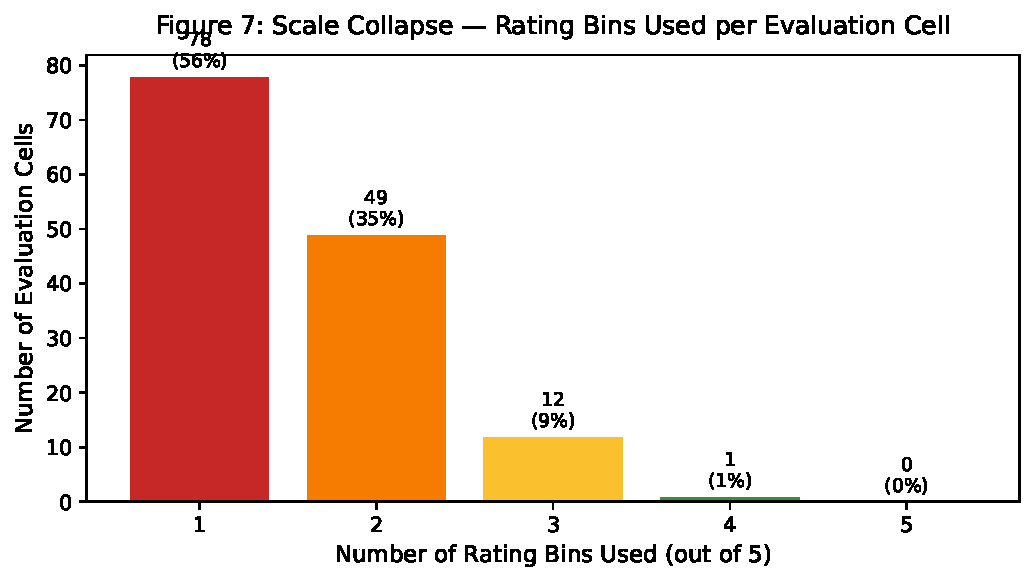
\includegraphics[width=0.85\linewidth]{fig7_scale_collapse_bins.pdf}
  \caption{Scale collapse --- number of rating bins used per evaluation cell.}
  \label{fig:bins}
\end{figure}

\begin{figure}[h]
  \centering
  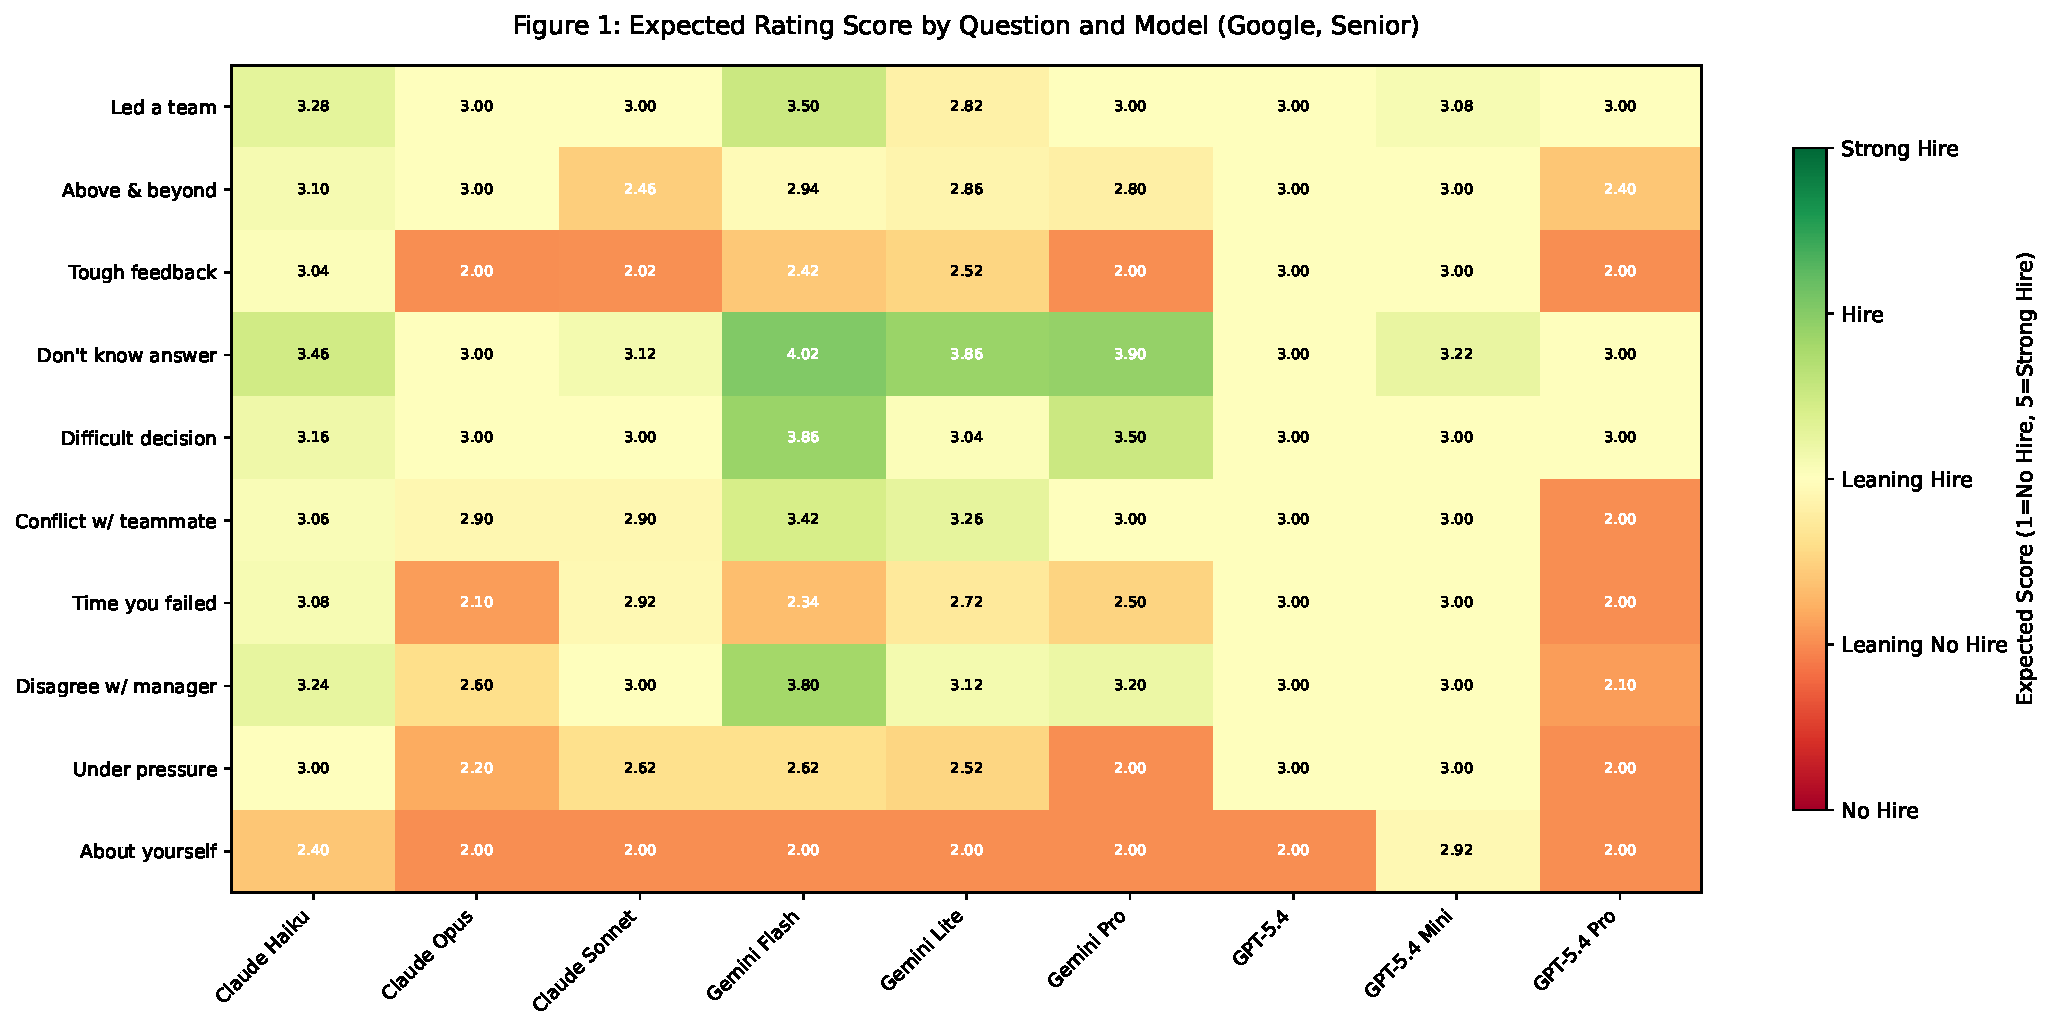
\includegraphics[width=0.95\linewidth]{fig1_scale_heatmap.pdf}
  \caption{Expected rating score by question and model (Google, Senior slice).}
  \label{fig:heatmap}
\end{figure}

Formal information-theoretic analysis confirms the severity: Shannon entropy is 0.707 nats against a maximum of 1.609 nats for a uniform 5-category distribution, yielding a \textbf{normalized entropy of only 0.439}. The effective number of categories ($\exp(H)$) is \textbf{2.03} --- a 5-point scale is functioning as a 2-point scale. The Gini-Simpson diversity index of 0.378 further corroborates that fewer than 2 categories carry meaningful probability mass.

\textbf{Implication.} The 5-point scale degenerates into a de facto binary judgment (Leaning No Hire vs.\ Leaning Hire) under LLM evaluation. There is \textbf{zero headroom to distinguish exceptional candidates from mediocre ones}, and no mechanism to flag clearly unqualified candidates. Any selection system built on these ratings is operating with far less discriminative power than its scale implies.

\subsection{Finding 2: Test--Retest Unreliability --- 10$\times$ Spread in Consistency}

\begin{figure}[h]
  \centering
  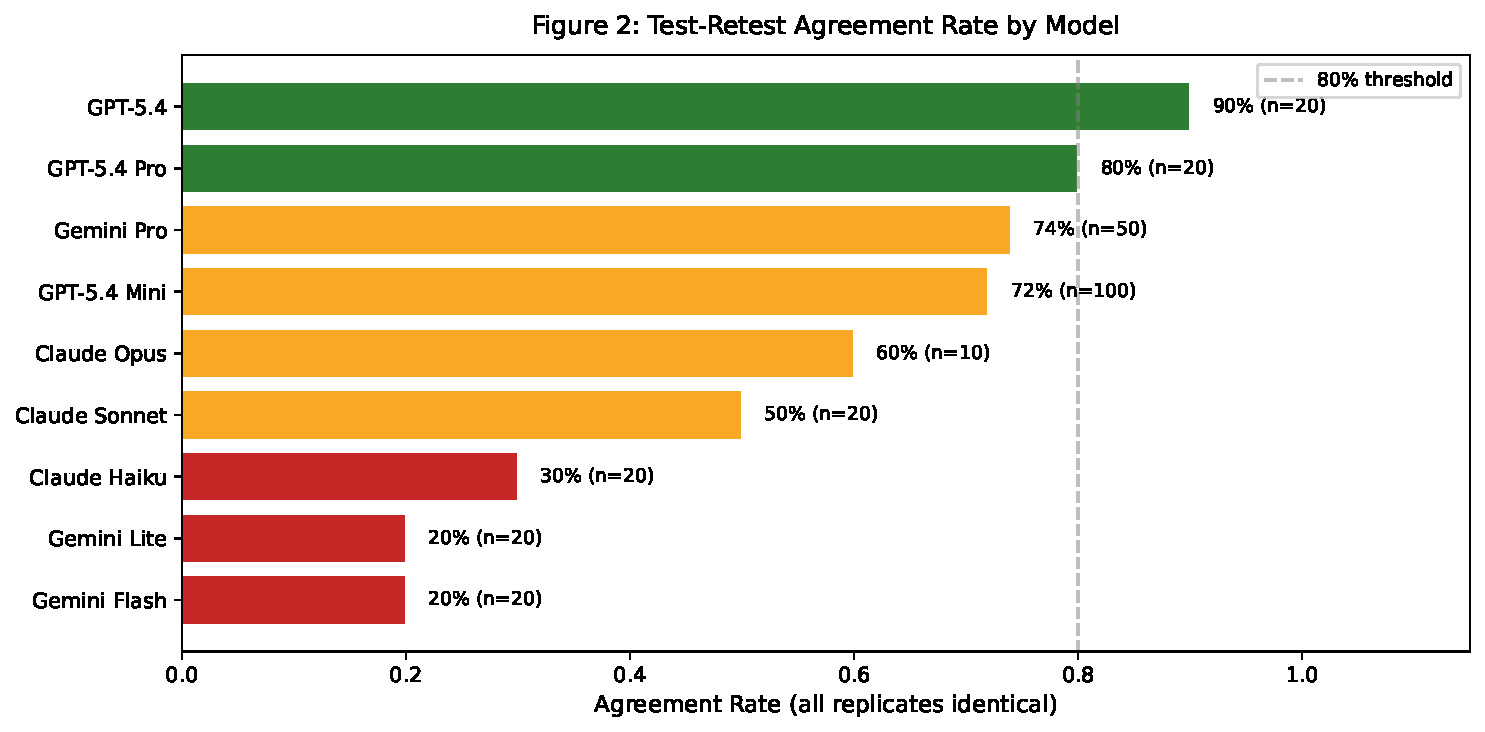
\includegraphics[width=0.9\linewidth]{fig2_test_retest.pdf}
  \caption{Test--retest agreement rate by model.}
  \label{fig:testretest}
\end{figure}

Test--retest reliability varies by an order of magnitude across models (Table~\ref{tab:testretest}). GPT-5.4 achieves perfect 100\% agreement in its best runs (identical ratings across all replicates). At the other extreme, Gemini Flash and Claude Haiku drop to 10--20\% agreement, with ordinal pstdev of 0.37--0.42 --- nearly a \textbf{full grade of jitter on a 5-point scale}.

\begin{table}[h]
\caption{Test--retest agreement and ordinal pstdev across runs.}
\label{tab:testretest}
\centering
\begin{tabular}{lccc}
\toprule
\textbf{Model} & \textbf{Best Run Agreement} & \textbf{Worst Run Agreement} & \textbf{Worst pstdev} \\
\midrule
gpt-5.4 & \textbf{1.00} (SD=0) & 0.80 & 0.08 \\
gpt-5.4-pro & 0.80 & 0.80 & 0.079 \\
gpt-5.4-mini & 0.80 & 0.60 & 0.147 \\
gemini-3.1-pro-preview & 0.90 & 0.60 & 0.20 \\
claude-haiku-4-5 & 0.50 & \textbf{0.10} & 0.421 \\
gemini-3-flash-preview & 0.20 & \textbf{0.20} & \textbf{0.369} \\
gemini-3.1-flash-lite & 0.30 & \textbf{0.10} & \textbf{0.381} \\
\bottomrule
\end{tabular}
\end{table}

Formal ICC(2,1) analysis (two-way random, single measures) quantifies the gap (Table~\ref{tab:icc}). ICC values range from 0.852 (gpt-5.4-pro) to 0.160 (claude-haiku-4-5) --- a \textbf{5.3$\times$ spread}. Only one model (gpt-5.4-pro) exceeds the conventional 0.75 threshold for ``good'' reliability~\cite{cicchetti1994}. Four models fall below the 0.50 ``fair'' threshold, with claude-haiku-4-5 approaching chance-level consistency. Notably, gpt-5.4-mini --- the highest-volume model in our benchmark (50 samples/cell) --- achieves only 0.342 despite having the most data to stabilize.

\begin{table}[h]
\caption{ICC(2,1) reliability per model.}
\label{tab:icc}
\centering
\begin{tabular}{lcc}
\toprule
\textbf{Model} & \textbf{ICC(2,1)} & \textbf{Interpretation} \\
\midrule
gpt-5.4-pro & \textbf{0.852} & Good reliability \\
claude-opus-4-6 & 0.756 & Moderate-to-good \\
gpt-5.4 & 0.753 & Moderate-to-good \\
gemini-3.1-pro-preview & 0.737 & Moderate \\
gemini-3-flash-preview & 0.734 & Moderate \\
claude-sonnet-4-6 & 0.691 & Moderate \\
gemini-3.1-flash-lite & 0.655 & Moderate \\
gpt-5.4-mini & 0.342 & Poor \\
claude-haiku-4-5 & \textbf{0.160} & Poor --- near random \\
\bottomrule
\end{tabular}
\end{table}

\textbf{Implication.} A candidate evaluated by Gemini Flash could receive ``Leaning Hire'' on one submission and ``Leaning No Hire'' on the next, purely from stochastic variation. \textbf{Single-shot LLM scores are unreliable for low-consistency models. Repeatability must be benchmarked and reported before deployment.}

\subsection{Finding 3: Inter-Model Disagreement --- Swapping Models Reshuffles Rankings}

\begin{figure}[h]
  \centering
  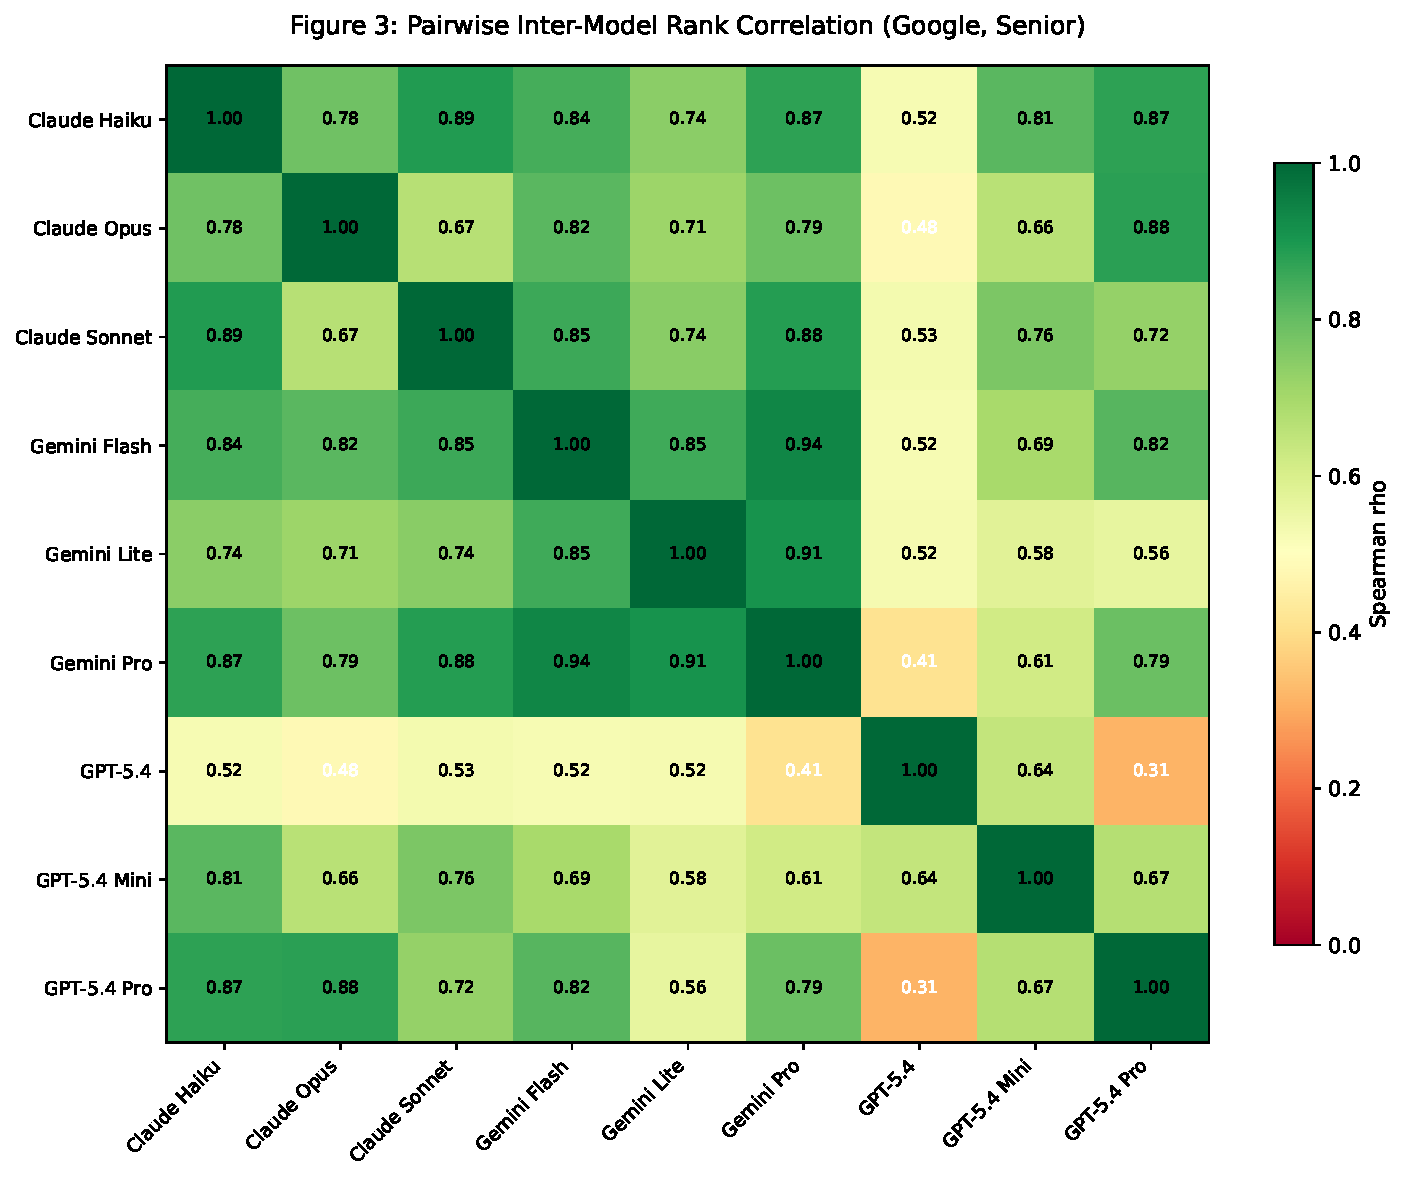
\includegraphics[width=0.85\linewidth]{fig3_spearman_heatmap.pdf}
  \caption{Pairwise inter-model rank correlation (Google, Senior).}
  \label{fig:spearman}
\end{figure}

Pairwise Spearman rank correlations of per-question expected scores reveal striking disagreement patterns (Table~\ref{tab:spearman}). The most surprising finding: \textbf{same-brand variant agreement ($\rho=0.25$--$0.31$) can be worse than cross-vendor agreement ($\rho=0.52$--$0.87$)}. Upgrading from GPT-5.4 to GPT-5.4-pro --- ostensibly a capability improvement within the same product line --- can reshuffle candidate rankings more than switching to an entirely different vendor's model.

\begin{table}[h]
\caption{Selected pairwise Spearman rank correlations (Google, Senior).}
\label{tab:spearman}
\centering
\begin{tabular}{lcc}
\toprule
\textbf{Model Pair} & \textbf{Spearman $\rho$} & \textbf{Interpretation} \\
\midrule
Gemini 3 Flash $\leftrightarrow$ Gemini 3.1 Pro & \textbf{0.936} & Same-family, excellent \\
Claude Haiku $\leftrightarrow$ Claude Sonnet & \textbf{0.890} & Same-family, excellent \\
Claude Haiku $\leftrightarrow$ Gemini 3.1 Pro & 0.874 & Cross-family, good \\
Gemini 3 Flash $\leftrightarrow$ GPT-5.4 & 0.522 & Moderate only \\
GPT-5.4 $\leftrightarrow$ GPT-5.4-pro & \textbf{0.314} & Same-brand, near-random \\
GPT-5.4 $\leftrightarrow$ GPT-5.4-pro (mid-level) & \textbf{0.249} & Lowest --- effectively random \\
\bottomrule
\end{tabular}
\end{table}

Three formal tests confirm that inter-model disagreement is both statistically significant and substantively large:
\begin{enumerate}
  \item \textbf{Friedman test} ($\chi^2 = 35.56$, $p = 2.8\times10^{-5}$, $k=9$ models, $n=10$ questions): Models produce significantly different rating distributions. Mean rank analysis reveals gpt-5.4-pro as the harshest rater (mean rank $=2.05$) and claude-haiku-4-5 as the most lenient (mean rank $=7.9$) --- a 3.9$\times$ gap in rank position.
  \item \textbf{Kendall's $W = 0.639$} ($\chi^2 = 51.79$, $p<0.001$): Models show moderate concordance on question ranking --- they partly agree on which questions are ``harder'' versus ``easier,'' but agreement is far from complete. A $W$ of 0.639 indicates roughly 64\% shared ranking variance, leaving 36\% attributable to idiosyncratic model-specific difficulty calibration.
  \item \textbf{Krippendorff's $\alpha = 0.523$} (ordinal, 9 coders $\times$ 10 units): Inter-model agreement falls below the conventional 0.667 threshold for tentative conclusions~\cite{krippendorff2011} and far below the 0.800 threshold required for reliable coding. This means LLM ratings would \textbf{not pass inter-rater reliability standards} in any social-science content-analysis study.
\end{enumerate}

Furthermore, vulnerability-category questions (failure, conflict, pressure) show the highest cross-model standard deviation (up to 0.58), serving as the most potent amplifiers of inter-model disagreement. GPT-5.4-pro rates ``tough feedback'' and ``conflict'' questions at 100\% ``Leaning No Hire'' (expected score $=2.0$), while GPT-5.4-mini rates the identical questions at 100\% ``Leaning Hire'' (expected score $=3.0$) --- same brand, one full ordinal grade apart.

\textbf{Implication.} Swapping model versions is not a neutral operation. It is functionally equivalent to swapping the entire scoring rubric, with unpredictable effects on candidate rankings.

\subsection{Finding 4: Question-Type Sensitivity --- 2-Grade Swings from Question Framing}

\begin{figure}[h]
  \centering
  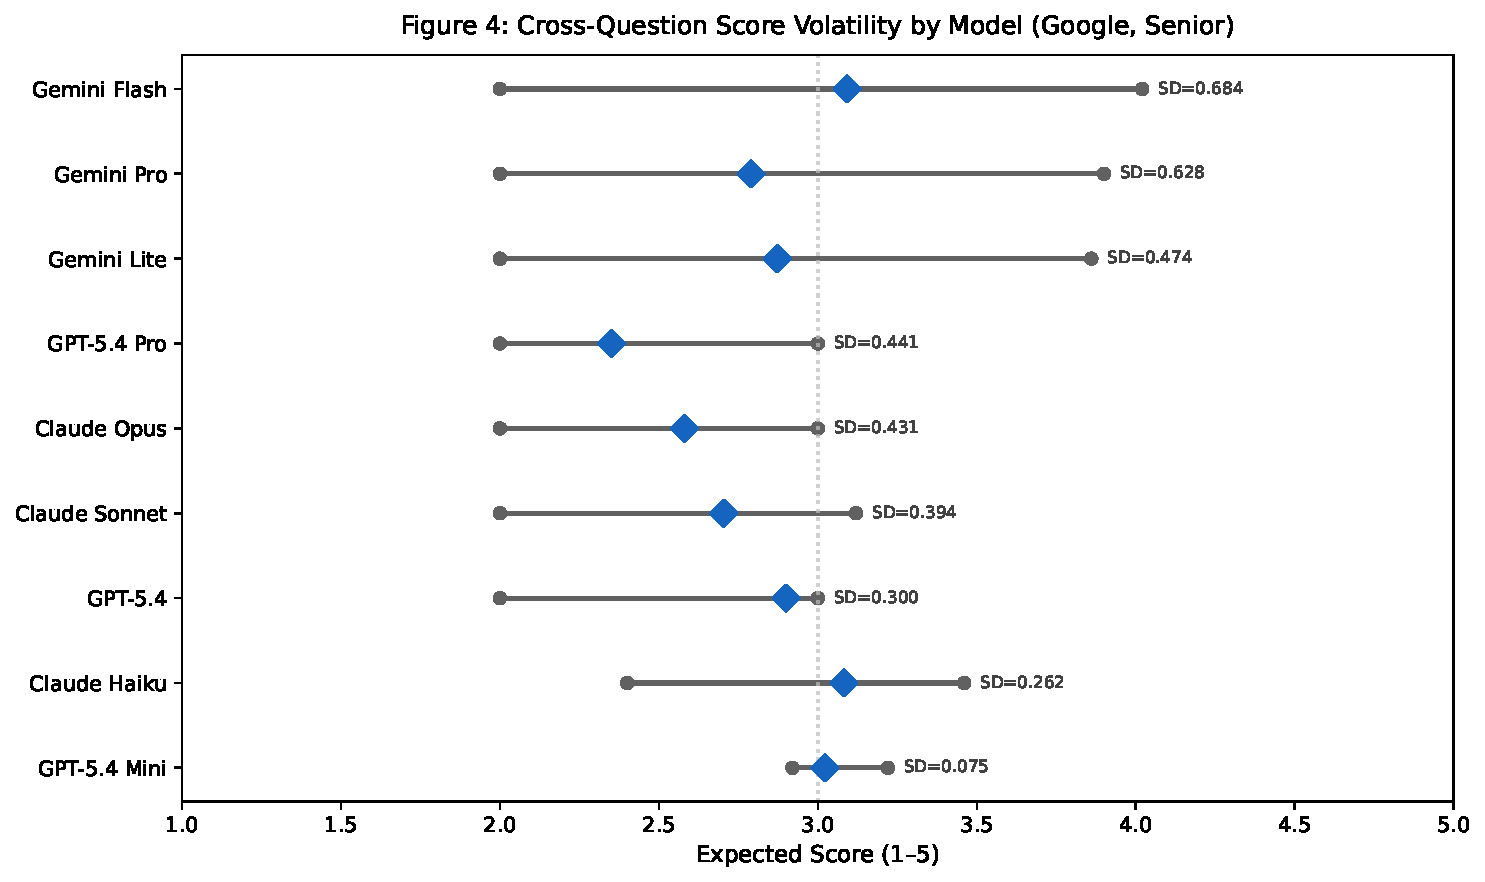
\includegraphics[width=0.9\linewidth]{fig4_cross_q_volatility.pdf}
  \caption{Cross-question score volatility by model (Google, Senior).}
  \label{fig:volatility}
\end{figure}

The same candidate answer receives dramatically different ratings depending on question type:
\begin{itemize}
  \item \textbf{``Tell me about yourself''} (Google, Senior): 8 out of 11 models assign 100\% ``Leaning No Hire'' (expected score $=2.0$).
  \item \textbf{``How do you handle not knowing the answer?''}: Gemini Flash assigns 98\% ``Hire'' (expected score $=4.02$).
\end{itemize}

This represents a \textbf{2-full-ordinal-point difference} (2.0 vs.\ 4.0) for the same candidate, purely based on question framing. Cross-question expected score standard deviation ranges from 0.075 (GPT-5.4-mini, near-flat) to 0.684 (Gemini Flash, highly volatile) --- a 9$\times$ gap in sensitivity.

\textbf{Implication.} LLM ``harshness'' is strongly governed by question type. Cross-question candidate comparison requires normalization or stratification. A candidate who excels at ``how do you handle X'' questions but struggles with ``tell me about a time you failed'' may be rated identically to a candidate with the opposite profile --- or dramatically differently, depending on which model is used.

\subsection{Finding 5: Expectation Gap --- Community ``Best Answers'' Score Below Hire}

\begin{figure}[h]
  \centering
  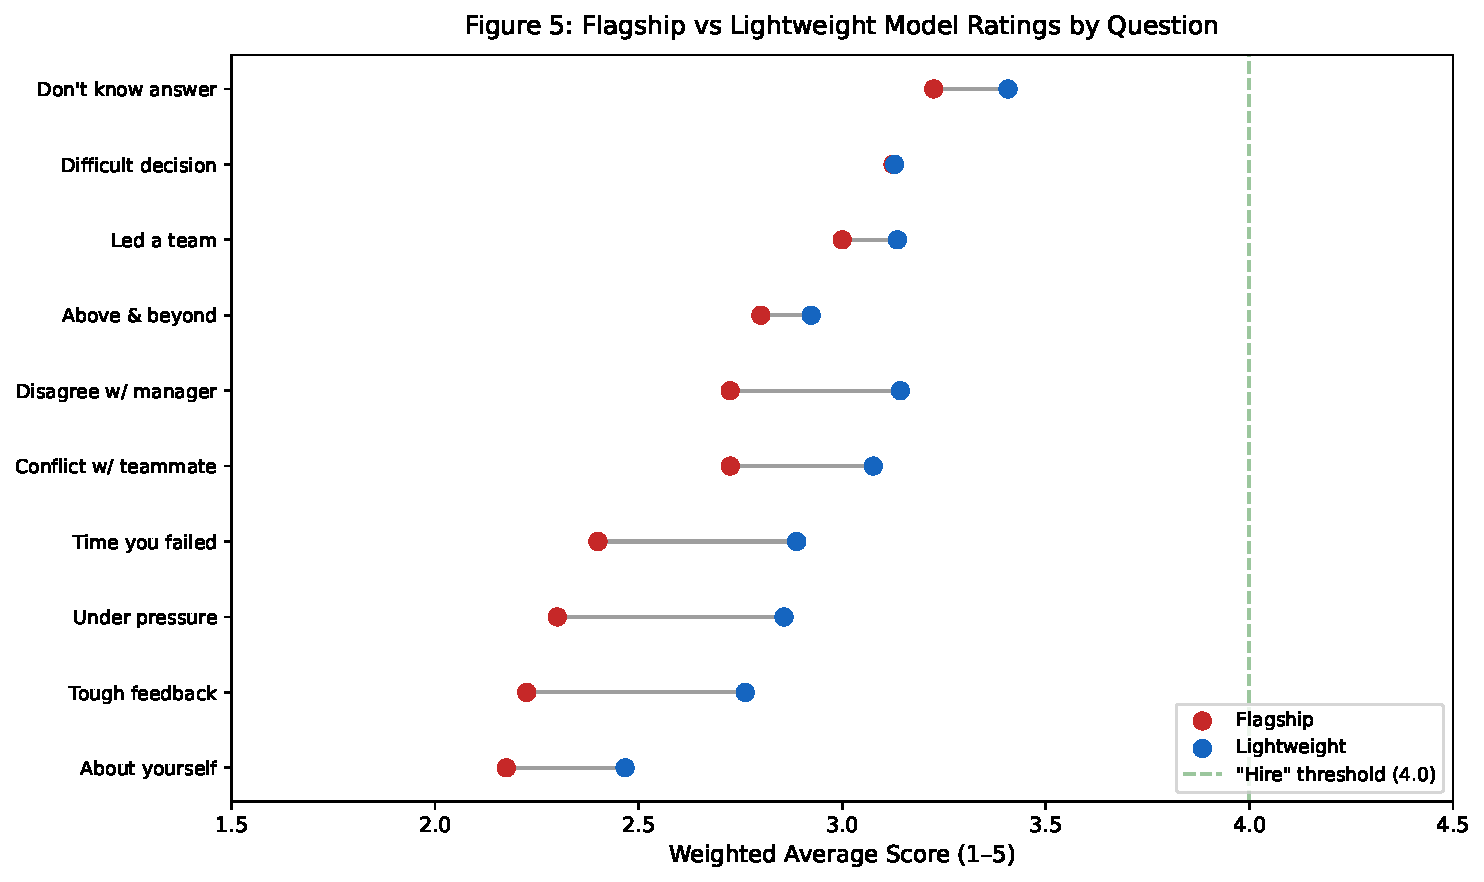
\includegraphics[width=0.9\linewidth]{fig5_tier_comparison.pdf}
  \caption{Flagship vs.\ lightweight model ratings by question.}
  \label{fig:tier}
\end{figure}

The 10 answers used in this experiment come from a repository with 8{,}000+ GitHub stars --- representing broad community endorsement. One would reasonably expect these answers to achieve at least ``Hire'' (4.0 on the 5-point scale).

\begin{table}[h]
\caption{Actual weighted-average ratings per question.}
\label{tab:ratings}
\centering
\begin{tabular}{lcc}
\toprule
\textbf{Question (abridged)} & \textbf{Flagship Avg} & \textbf{Lightweight Avg} \\
\midrule
Handle not knowing the answer & \textbf{3.23} & \textbf{3.41} \\
Difficult decision & 3.13 & 3.13 \\
Led a team & 3.00 & 3.14 \\
Above and beyond & 2.80 & 2.92 \\
Conflict with teammate & 2.73 & 3.08 \\
Disagreement with manager & 2.73 & 3.14 \\
Time you failed & 2.40 & 2.89 \\
Under pressure & 2.30 & 2.86 \\
Tough feedback & 2.23 & 2.76 \\
Tell me about yourself & \textbf{2.18} & \textbf{2.47} \\
\bottomrule
\end{tabular}
\end{table}

\textbf{Zero out of 10 questions reach the ``Hire'' threshold (4.0)} for either flagship or lightweight models. The best-performing question barely exceeds ``Leaning Hire'' (3.0). Flagship models are consistently harsher than lightweight models (all 10 differences negative, mean $\Delta = -0.31$).

A Wilcoxon signed-rank test confirms that the flagship--lightweight gap is statistically significant: $W=0$, $z=-2.80$, $p=0.005$ ($n=10$ matched question pairs, all 10 differences non-zero and negative). The mean flagship rating (2.67) is 0.31 ordinal points below the mean lightweight rating (2.98). This is not random fluctuation --- \textbf{larger, more ``capable'' models are systematically harsher evaluators}, a finding with direct implications for organizations that assume upgrading model tier improves evaluation quality.

This expectation gap admits two non-mutually-exclusive explanations:
\begin{enumerate}
  \item \textbf{The internet is not the interview room} --- Even highly upvoted community BQ answers may not meet actual interview ``Hire'' standards. Star count reflects ``sounds reasonable'' crowd consensus, not calibrated interview quality.
  \item \textbf{SOTA LLMs are still unreliable for BQ evaluation} --- Current frontier models may be systematically too harsh or unable to reliably distinguish strong behavioral answers from mediocre ones.
\end{enumerate}

\textbf{Implication.} Neither crowd-sourced BQ prep materials nor LLM evaluators should be trusted at face value without validation against human interviewer ground truth.

\subsection{Summary of Formal Statistical Tests}

Table~\ref{tab:tests} consolidates the formal statistical tests applied across the five findings. All tests point to the same conclusion: LLM behavioral interview ratings exhibit statistically significant unreliability across every measured dimension --- scale utilization, test--retest consistency, inter-model agreement, and tier-level bias.

\begin{table}[h]
\caption{Summary of formal statistical tests.}
\label{tab:tests}
\centering
\small
\begin{tabular}{llllp{4.3cm}}
\toprule
\textbf{Test} & \textbf{Statistic} & \textbf{Value} & \textbf{$p$-value} & \textbf{Interpretation} \\
\midrule
Scale utilization (entropy) & $H/H_{max}$ & 0.707 / 1.609 nats & --- & Normalized entropy = 0.44; effective categories = 2.03 \\
Friedman test & $\chi^2(8)$ & 35.56 & $2.8\times10^{-5}$ & Models give significantly different ratings \\
Kendall's $W$ & $W$ & 0.639 & $<0.001$ & Moderate concordance on question ranking \\
Krippendorff's $\alpha$ (ordinal) & $\alpha$ & 0.523 & --- & Below 0.667 tentative-conclusion threshold \\
ICC(2,1) range & ICC & 0.160--0.852 & --- & Poor to good; only 1/9 models above 0.75 \\
Wilcoxon signed-rank & $z$ & $-2.803$ & 0.005 & Flagship harsher than lightweight \\
\bottomrule
\end{tabular}
\end{table}

\section{Model Robustness Scorecard: Stability and Consensus Are Orthogonal}\label{sec:scorecard}

\begin{figure}[h]
  \centering
  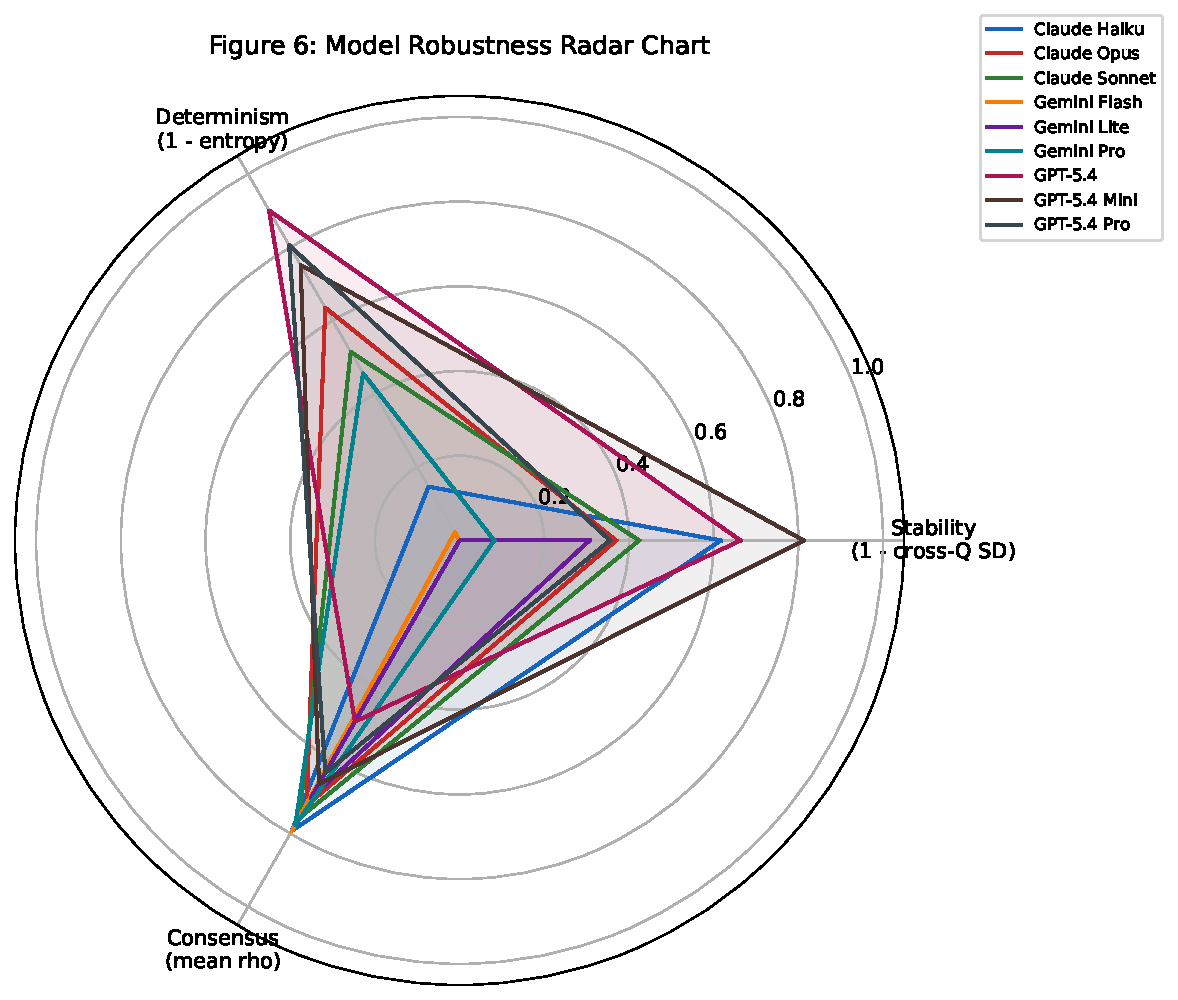
\includegraphics[width=0.7\linewidth]{fig6_robustness_radar.pdf}
  \caption{Model robustness radar chart.}
  \label{fig:radar}
\end{figure}

Aggregating all metrics per model reveals that \textbf{stability} (self-consistency) and \textbf{consensus} (agreement with other models) are independent dimensions (Table~\ref{tab:scorecard}).

\begin{table}[h]
\caption{Model robustness scorecard. Lower Cross-Q SD and entropy are better; higher mean $\rho$ is better.}
\label{tab:scorecard}
\centering
\small
\begin{tabular}{lcccp{4.5cm}}
\toprule
\textbf{Model} & \textbf{Cross-Q SD} & \textbf{Entropy} & \textbf{Mean $\rho$} & \textbf{Profile} \\
\midrule
gpt-5.4-mini & \textbf{0.13} & 0.12 & 0.66 & Most stable, moderate consensus \\
gpt-5.4 & 0.23 & \textbf{0.05} & \textbf{0.49} & Ultra-deterministic, lowest consensus \\
claude-haiku-4-5 & 0.26 & 0.43 & \textbf{0.79} & Balanced, highest consensus (tied) \\
claude-sonnet-4-6 & 0.39 & 0.24 & 0.76 & Mid-range \\
claude-opus-4-6 & 0.43 & 0.18 & 0.72 & Mid-range \\
gpt-5.4-pro & 0.44 & 0.10 & 0.63 & Deterministic but cross-Q volatile \\
gemini-3.1-flash-lite & 0.47 & \textbf{0.50} & 0.70 & Noisiest distribution \\
gemini-3.1-pro & 0.63 & 0.27 & 0.78 & Volatile, good consensus \\
gemini-3-flash & \textbf{0.68} & 0.49 & \textbf{0.79} & Most volatile, highest consensus (tied) \\
\bottomrule
\end{tabular}
\end{table}

The key insight: \textbf{GPT-5.4 is ``confidently idiosyncratic''} --- it produces near-deterministic outputs (entropy $=0.05$) but agrees least with other models ($\rho=0.49$). Conversely, \textbf{Gemini Flash is ``volatile but mainstream''} --- it has the highest cross-question variance (SD $=0.68$) yet ties for the highest inter-model consensus ($\rho=0.79$).

No single model dominates all robustness dimensions. Choosing a model for hiring evaluation requires explicit trade-offs between self-consistency and inter-model alignment --- a decision that most current deployments do not make transparently.

\section{Discussion}\label{sec:discussion}

\subsection{A Minimum Reliability Checklist for LLM Interview Evaluators}

Based on our findings, we propose that any deployment of LLM interview evaluators should meet the following minimum reliability requirements (Table~\ref{tab:checklist}).

\begin{table}[h]
\caption{Proposed minimum reliability checklist for LLM interview evaluators.}
\label{tab:checklist}
\centering
\small
\begin{tabular}{llllp{2.8cm}}
\toprule
\textbf{Requirement} & \textbf{Metric} & \textbf{Threshold} & \textbf{Our Result} & \textbf{Finding} \\
\midrule
R1: Scale utilization & Normalized entropy & $\geq 0.60$ & \textbf{0.44}~\textsc{fail} & F1: 2.03 effective categories \\
R2: Test--retest stability & ICC(2,1) & $\geq 0.75$ & \textbf{0.16--0.85} (1/9 pass)~\textsc{fail} & F2: 5.3$\times$ ICC spread \\
R3: Cross-model robustness & Krippendorff's $\alpha$ & $\geq 0.667$ & \textbf{0.523}~\textsc{fail} & F3: Below tentative threshold \\
R4: Question-type fairness & Cross-Q score SD & $\leq 0.30$ & \textbf{0.075--0.684}~\textsc{fail} & F4: 9$\times$ spread \\
R5: Calibration validity & Correlation w/ humans & $\geq 0.60$ & N/A & F5: Expectation gap \\
\bottomrule
\end{tabular}
\end{table}

Currently, \textbf{no model in our benchmark simultaneously meets all five requirements}:
\begin{itemize}
  \item GPT-5.4-mini comes closest (4/5), failing only on R5 (no human ground truth available).
  \item Several models fail R1, R2, or R3 individually.
\end{itemize}

\subsection{Implications for AI Hiring Policy}

\textbf{For NYC Local Law 144 compliance.} The law requires annual bias audits, but our results suggest that reliability auditing (test--retest, inter-model) should be equally mandatory. A system that gives different ratings to the same candidate on different days fails a basic fairness standard regardless of aggregate bias statistics.

\textbf{For EU AI Act compliance.} High-risk AI systems must demonstrate ``accuracy, robustness, and cybersecurity.'' Our test--retest results (10--20\% agreement for some models) and inter-model disagreement ($\rho=0.25$ for same-brand variants) directly challenge robustness claims.

\textbf{For EEOC guidance.} If a candidate's hiring outcome depends more on which model version is used ($\rho=0.25$ between GPT-5.4 and GPT-5.4-pro) than on their actual answer quality, this constitutes a form of arbitrary discrimination that current anti-discrimination frameworks are ill-equipped to address.

\subsection{Implications for LLM-as-Judge Research}

Our findings extend the LLM-as-Judge literature in several important ways:
\begin{enumerate}
  \item \textbf{Domain-specific failure modes:} Scale collapse appears to be particularly severe in the hiring domain, where the 5-point scale has only 2 meaningful categories. This may not manifest in general NLG evaluation tasks.
  \item \textbf{Cross-version instability:} The finding that same-brand model variants ($\rho=0.25$) disagree more than cross-vendor pairs ($\rho=0.87$) has implications for any system that relies on a specific model checkpoint. Model updates can silently invalidate evaluation pipelines.
  \item \textbf{Orthogonality of stability and consensus:} The independence of self-consistency and inter-model agreement is a novel finding that suggests current model selection practices (choosing the ``most capable'' model) may be misguided for evaluation tasks.
\end{enumerate}

\subsection{Implications for Job Seekers}
\begin{enumerate}
  \item \textbf{Do not assume fairness:} The same answer can receive ratings differing by 2 full grades depending on model choice and question type.
  \item \textbf{Resubmission may yield different results:} For low-consistency models, re-taking the same assessment can change outcomes purely from stochastic variation.
  \item \textbf{Community preparation materials may not calibrate correctly:} High-star GitHub answers still score below ``Hire'' under LLM evaluation.
\end{enumerate}

\subsection{Why This Matters for the United States}
AI-assisted hiring is projected to affect over 100 million job applications annually in the United States~\cite{levy2025}. The reliability failures documented in this paper --- scale collapse masking discriminative power, test--retest jitter exceeding one full grade, inter-model disagreement rivaling random assignment --- have direct consequences for labor market efficiency and worker welfare. Unreliable AI hiring tools waste employer resources on false-positive screenings and systematically disadvantage candidates through arbitrary scoring variation. Our findings provide the empirical foundation for evidence-based regulation of AI hiring tools, supporting the goals of the EEOC, NIST AI RMF, and state-level AI hiring legislation.

\section{Limitations}\label{sec:limitations}
\begin{enumerate}
  \item \textbf{Answer source:} Our answers come from a community-curated GitHub repository rather than real interview recordings. While this provides a useful community-consensus baseline, real candidate answers may exhibit different characteristics (nervousness, digressions, varied articulation quality) that could affect LLM evaluation patterns.
  \item \textbf{No human ground truth:} We lack parallel human interviewer ratings for the same answers. While Finding~5 (Expectation Gap) provides indirect calibration evidence, direct human--LLM agreement measurement remains future work.
  \item \textbf{Behavioral interviews only:} Our audit covers behavioral (competency-based) interview questions only. Technical interviews, system design interviews, and case study formats may exhibit different reliability patterns.
  \item \textbf{Model snapshot:} LLM capabilities change with model updates. Our results reflect model behavior at the time of experimentation (March 2026). Findings should be periodically revalidated as models evolve.
  \item \textbf{Single answer per question:} We evaluate one community-sourced answer per question. A more comprehensive benchmark would include multiple answers of varying quality per question to test discriminative validity.
  \item \textbf{Prompt sensitivity:} While we use a standardized prompt, different prompt designs could yield different reliability profiles. Our findings represent one specific --- but realistic --- evaluation prompt template.
\end{enumerate}

\section{Conclusion}\label{sec:conclusion}

We present the first systematic reliability audit of LLM behavioral interview scoring, evaluating 9 frontier models across 141 evaluation cells. Our five core findings --- scale collapse, test--retest unreliability, inter-model disagreement, question-type sensitivity, and expectation gap --- collectively demonstrate that \textbf{current LLM interview evaluators fail basic psychometric reliability standards}.

The most concerning finding is that these failures are not merely theoretical: they occur at the frontier of LLM capability, across all three major model families, and on the most widely-used behavioral interview preparation materials on the internet. Scale collapse means the rating instrument lacks discriminative power. Test--retest jitter means outcomes are partially random. Inter-model disagreement means outcomes depend on vendor choice. Question-type sensitivity means outcomes depend on question framing. The expectation gap means the evaluator's standards may not reflect human judgment.

Any LLM-based interview scoring system that reports only point estimates without cross-question variance, inter-model rank correlation, and test--retest metrics is \textbf{masking real noise with false precision}. We urge practitioners, policymakers, and researchers to adopt the minimum reliability checklist proposed in this paper before deploying LLM evaluators in hiring contexts.

\bibliographystyle{plainnat}
\bibliography{references}

\appendix

\section{Experimental Configuration Details}

\subsection{System Configuration}
\begin{itemize}
  \item \textbf{Python Version:} 3.11+
  \item \textbf{LLM Integration:} LiteLLM library
  \item \textbf{Async Processing:} asyncio with max 5 concurrent requests
  \item \textbf{Experiment Dates:} March 25--27, 2026
\end{itemize}

\subsection{Model Access}
All models accessed via LiteLLM unified API. API keys stored in environment variables; no secrets committed to repository.

\subsection{Data and Code Availability}
The complete evaluation framework, analysis scripts, and raw experimental data are available at the project repository. The answer source is publicly available at \url{https://github.com/ashishps1/awesome-behavioral-interviews}.

\section{Supplementary Tables}

\subsection{Full Rating Distribution by Cell}
See \texttt{viz\_rating\_stats\_summary.csv} in supplementary materials for complete per-cell rating distributions across all 141 evaluation cells.

\subsection{Full Pairwise Spearman Correlation Matrix}
See \texttt{reliability\_pairwise\_spearman.csv} for all model-pair correlations stratified by company and level.

\subsection{Test--Retest Detail}
See \texttt{reliability\_rep\_per\_group.csv} and \texttt{reliability\_rep\_summary\_by\_run\_model.csv} for detailed replicate-level agreement data.

\end{document}
